\begin{frame}{A Theory of Onset Temperature in 2D: The Bound Dipole-Pair State}
% \begin{columns}
% \begin{column}{0.5\linewidth}
% \begin{itemize}
%     \item T
% \end{itemize}
% \end{column}

% \begin{column}{0.5\linewidth}
\begin{figure}
\begin{overprint}

\onslide<2>\centering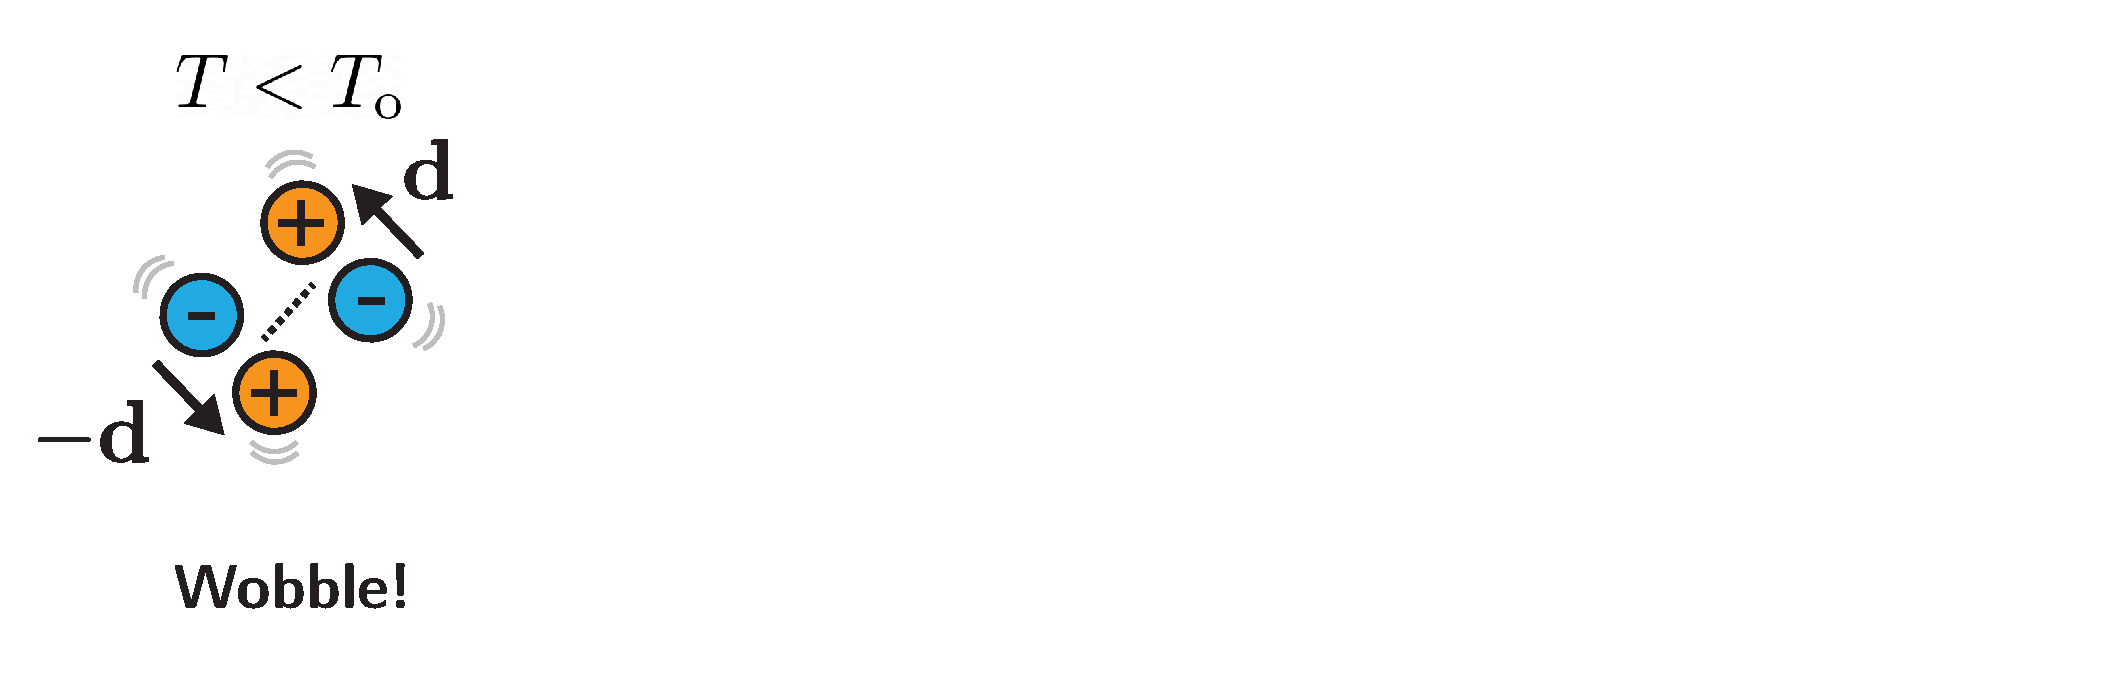
\includegraphics[width=0.65\linewidth]{4.d-kt_energyentropy/dofs_quadrupole-0.pdf}
%\caption{Testing}

\onslide<3>\centering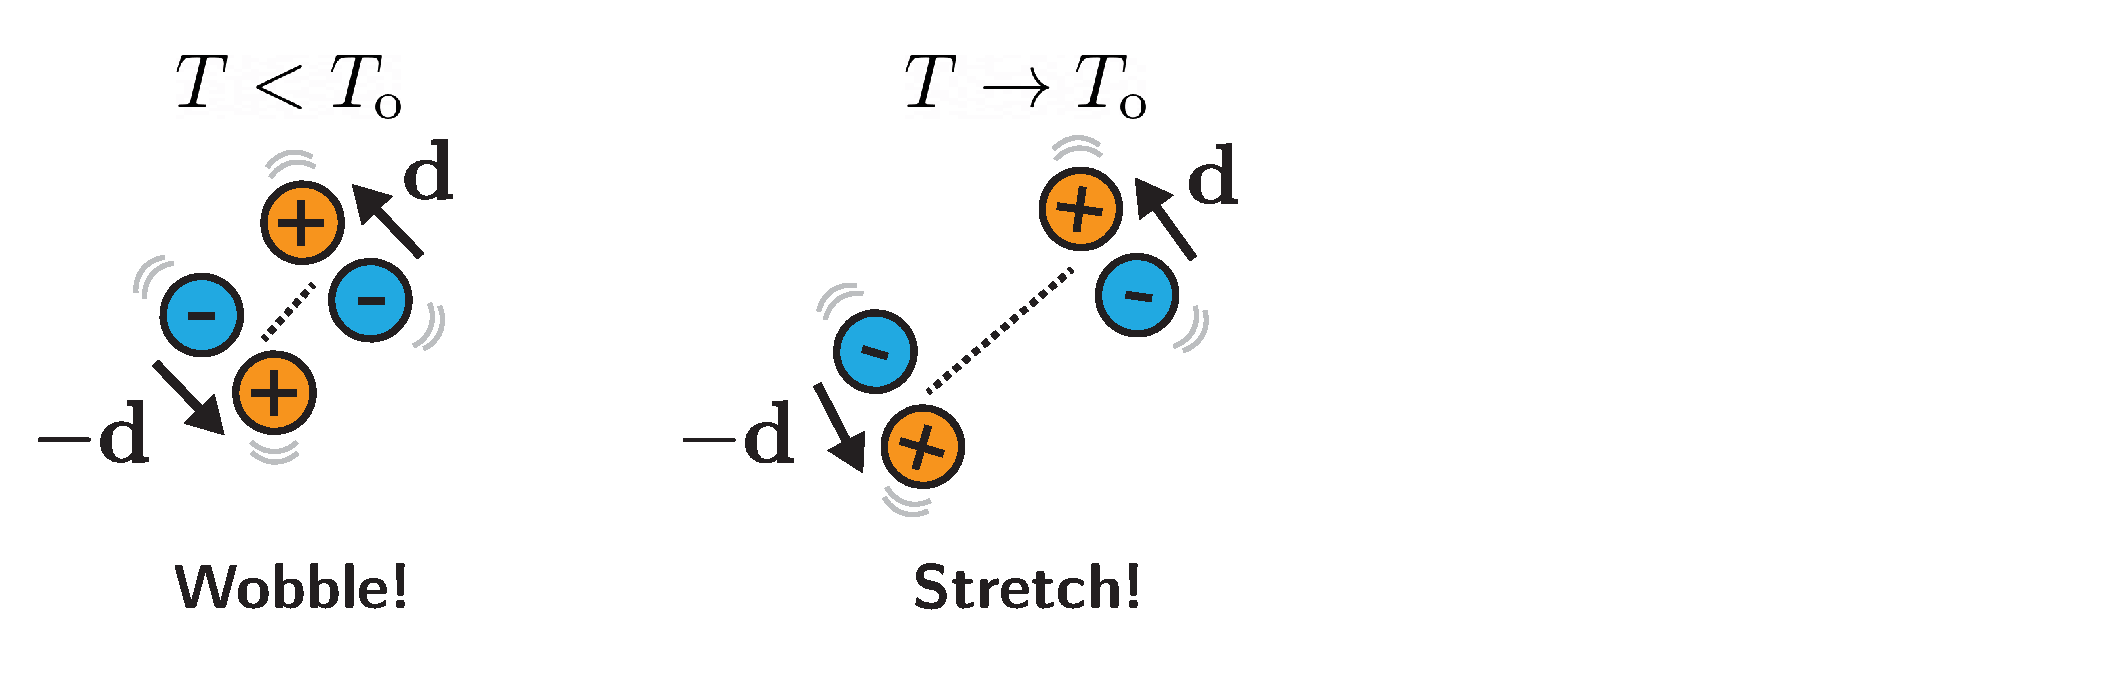
\includegraphics[width=0.65\linewidth]{4.d-kt_energyentropy/dofs_quadrupole-1.pdf}
%\caption{Testing}

\onslide<4->\centering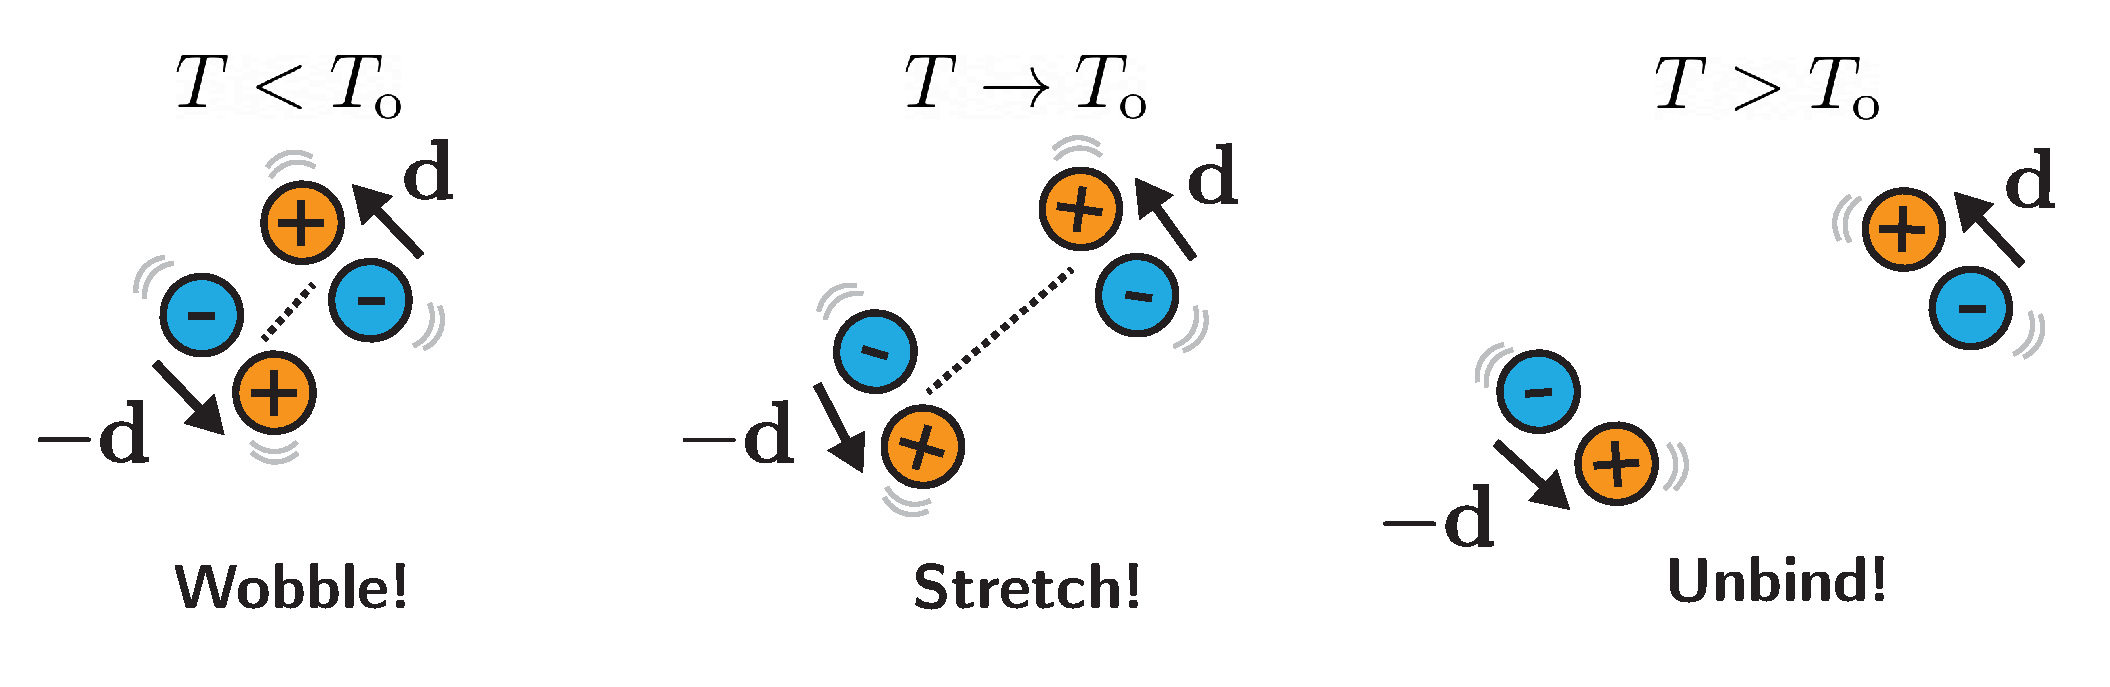
\includegraphics[width=0.65\linewidth]{4.d-kt_energyentropy/dofs_quadrupole-3.pdf}

\end{overprint}
    
\end{figure}

\vspace{-10pt}

\begin{itemize}
\item<1-> A localized excitation has internal degrees of freedom (rotation + stretching)
\begin{equation*}
\onslide<5->{\underbrace{\Delta F_\mathrm{f}}_{\substack{\text{Free energy of} \\ \text{formation}}} = \underbrace{ \frac{d_{\mathrm{c}}^{2} Y^{\mathrm{IS}}}{8 \pi} \ln \left(\frac{R}{R_{\mathrm{exc}}}\right) }_{\substack{\text{Elastic energy cost}}}} \onslide<6->{-\underbrace{2 k_\mathrm{B} T \ln \left(\sqrt{2 \pi} \frac{R}{R_\mathrm{exc}} \right)}_{\substack{\text{Entropy gain} }}}
\end{equation*}
\vspace{-9pt}
\item<7-> \textbf{The binding-unbinding transition ($\km{\beta_\mathrm{KT} Y^\mathrm{IS} d_\mathrm{c}^2 = 16 \pi}$):} bound-dipole pairs $\leftrightarrow$ free dipoles. 
\item<8->{Similar to the Kosterlitz-Thouless-Halperin-Nelson-Young (KTHNY) theory of dislocation-mediated melting\only<8->{\footnote{ Kosterlitz and Thouless, \textit{J. Phys. C} (1972); Kosterlitz and Thouless, \textit{J. Phys. C} (1973); Halperin and Nelson, \textit{Phys. Rev. Lett.} (1978); Nelson, \textit{Phys. Rev. B} (1978); Nelson and Halperin, \textit{Phys. Rev. B} (1979); Young, \textit{Phys. Rev. B} (1979)}}}.

\end{itemize}
\vspace{8pt}
% \end{column}

% \end{columns}


    
\end{frame}